\documentclass[11pt, a4paper]{jsarticle}
\usepackage{multicol}  % パッケージの追加
\usepackage[dvipdfmx]{graphicx}
\begin{document}
%=============================================================
%=============================================================
\section{Expandig laser beam}
\subsection*{Purpose}
実験の目的はビームの広がり角を求めることと,ビームエキスパンダーの製作,拡大率の評価である.
\subsection{Divergence of beam}
\subsubsection{Procedure}
まずビームホルダーを調節してビーム光が机に対して平行になるように調節する.
次に方眼紙によってスクリーンを製作してスクリーンからレーザーまでの距離$z$とスクリーンに当たったレーザー光の半径$d(z)$を求める.
測定結果を式(\ref{eq:a})に代入して図 \ref{fig:one}に表すレーザーのビームウエスト($d_0$)と広がり角($\theta$)を導き出す.

\begin{equation}
    d^2(z) = d_0^2 + \theta^2z^2 \label{eq:a}
\end{equation}\\


\begin{figure}[htbp]
 \begin{minipage}{0.45\hsize}
  \begin{center}
   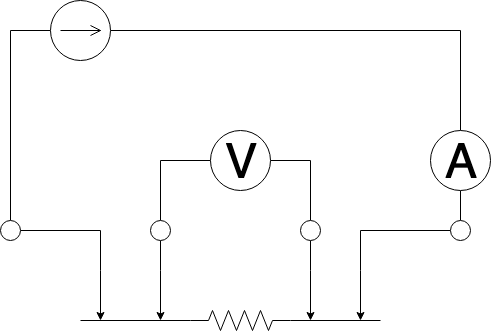
\includegraphics[width=60mm]{fig1.png}
  \end{center}
  \caption{ビームウエストと広がり角}
  \label{fig:one}
 \end{minipage}
 \begin{minipage}{0.45\hsize}
  \begin{center}
   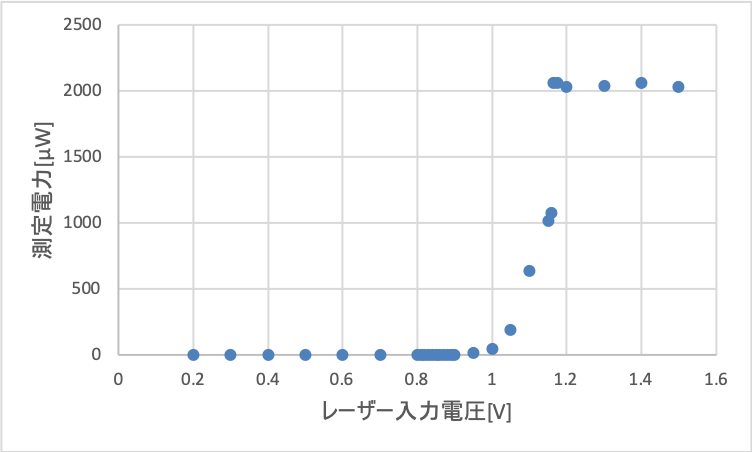
\includegraphics[width=60mm]{fig2.png}
  \end{center}
  \caption{$Distance$と$Diameter$}
  \label{fig:two}
 \end{minipage}
\end{figure}


そのため$d_0$,$\theta$を求めるためには,スクリーンに映し出されたレーザーの直径の値,レーザーの射出口からスクリーンまでの距離,二つの測定値が必要となるのでスクリーンからの距離が異なる二箇所で測定を行なった.

\newpage
\subsubsection{Result}
測定結果から次の表が得られた.
\begin{table}[htb]
  \begin{center}
    \caption{レーザーからスクリーンの距離と直径}
    \begin{tabular}{rrr} \hline
        $z(mm)$ & $d(z)(mm)$  \\ \hline
        500            & 1.1 \\
        4000           & 5.0 \\ \hline
    \end{tabular}
    \label{tab:a}
  \end{center}
\end{table}


またこの測定結果より,関係式(\ref{eq:a})において変数消去を行うことで$d_0 = 0.915mm$, $\theta = 1.22 \times 10 ^{-3}rad$
という値が得られた.
この結果よりレーザー光は確かに射出口から遠ざかれば遠ざかるほど広がっていることが確認できた.
一方でレーザーの広がり角は上記の通り非常に小さい角度であることが確認できた.
\subsubsection{Discussion}
通常実験用レーザーの広がり角は($mrad$)オーダーであるので今回の実験結果は実際の広がり角から大きずれることなく測定できたと考えられる.
しかし測定精度を下げる要因として,ビーム直径を測定する際にビームの強度が強すぎたために目視の正確さを欠いたことや,観測者が毎回入れ替わったことによりそれぞれの直径の定義がバラバラであったことなどが挙げられる.

そもそもビームの光はガウス分布に従うため正確な境目が存在しない.
したがってガウスシアンビームのビーム半径はビーム軸の上のピーク値の$1/e^2$まで減少する半径と決められている.
つまりビームの$0.135$倍暗くなっている所を境界と定めるべきであった.

また,この測定から得られた$\theta$,$d_0$の値はレーザー特有の値であり測定地点の変化によって変わるものではないので$Distance$,$Diameter$を2回ずつしか計測すればそれぞれの値を推測することは可能である.
一方で,$Distance$,$Diameter$の測定回数を増やすことでよりビームウエストと広がり角の値をより正確に測定することができると考えられる.
また今回の実験では$\theta$,$d_0$の値を求める際にスクリーンからの距離を二箇所のみ測定して関係式(\ref{eq:a})において連立して求めたがスクリーンからの距離を三箇所以上測定するとどの2点で計算するかが問題となってくる.
しかし前述の通り$\theta$,$d_0$の値はレーザー固有の値であるので測定回数を増やし正確に測定を行えば計算値は真の値に近づいていくことが予想される.

さらに光の強度を下げてビーム半径を測定しやすくするためにNDフィルターを利用して測定を行うなどの改善策が挙げられる.
%=============================================================
\subsection{The Keplerian Beam Expander}
\subsubsection{Procedure}
今回はケプラー型のビームエキスパンダーを製作する.
ケプラー型ビームエキスパンダーは凸レンズを二個組み合わせて製作する.
図\ref{fig:three}に示すように光学系を組み立てた.
まずNDフィルター($1\%\times2,25\%$)3枚をレーザーの前に置き,次に焦点距離$50mm$の凸レンズ,さらに置焦点距離$200mm$の凸レンズを置いた.
次に二つ目のレンズを抜けた光が平行光となるようにレンズの位置を調整した.
さらにエキスパンダーの拡大率を計算するために一つ目のレンズを透過する前のビーム直径,二つ目のレンズを透過した後のビーム直径をそれぞれ計測し,実際の拡大率と理論値との比較を行った.
\begin{figure}[htbp]
 \begin{center}
  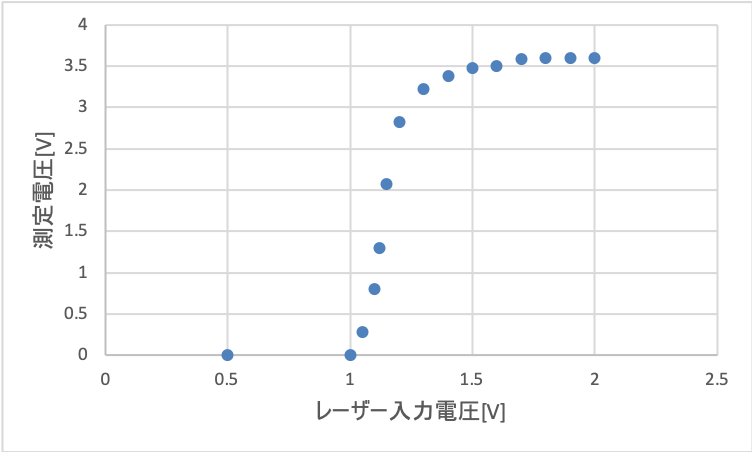
\includegraphics[width=100mm]{fig3.png}
 \end{center}
 \caption{ケプラー型ビームエキスパンダー}
 \label{fig:three}
\end{figure}

\subsubsection{Result}
二つ目のレンズを透過した光が平行光となったのはレンズ間距離$f_i + f_o$が$260mm$となった時であった.
またエキスパンダー入射前のビーム直径は$1.3mm$に対してエキスパンダーの透過光は$5.0mm$となりビームエキスパンダーを通ることでビーム半径が大きくなることが確認された.この時の拡大率は$3.85$であった.
\subsubsection{Discussion}
実験で使用した凸レンズは$f_i = 50mm$,$f_o = 200mm$だったので理論値としてはレンズ間の距離は$250mm$であるはずだが実験値はその値よりも大きい値となった.ビームの軌跡がレンズの中心に当たっていなかったために実際の焦点距離よりも実験値の焦点距離が大きくなってしまったなどが考えられる.
また拡大率が理論値の4倍よりも小さく出てしまった原因についても上記と同様のことが考えられる.この場合拡大率が理論値よりも小さくなったので焦点距離50mmの凸レンズの計測値がビームが中心に当たっていなかったなどの理由で実際の値よりも小さく出てしまったことが考えられる.そのように考えると平行光を作り出す時のレンズ間距離が理論値よりも大きくなってしまったことにも説明がつく.
%=============================================================
\subsection{The Galilean Beam Expander}
\subsubsection{Procedure}
図\ref{fig:four}に示すように光学系を組み立てた.
まず前回同様,NDフィルター($1\%\times2,25\%$)3枚をレーザーの前に置いた.
次に焦点距離$-40mm$の凹レンズを置き,その後で前回使用した焦点距離$200mm$の凸レンズを置いた.
次にエキスパンダーの透過光が平行光となるようにレンズ間の距離を調節した.
またエキスパンダーの透過光のビーム直径を測定し,透過前のビームと直径と比べて拡大率を計算し,理論値との違いを比べた.
\begin{figure}[htbp]
 \begin{center}
  \includegraphics[width=100mm]{fig4.png}
 \end{center}
 \caption{ガリレオ型ビームエキスパンダー}
 \label{fig:four}
\end{figure}
\subsubsection{Result}
エキスパンダーの透過光が平行光になる時のレンズ間の距離は$160mm$であり理論値と一致した.
また,エキスパンダー透過前のビーム直径は$1.5mm$であったのに対して,エキスパンダーを通った後のビーム直径は$7.5mm$であった.
以上より実験での拡大率は$5.0$でありこれも理論値と一致した.
\subsubsection{Discussion}
今回の実験ではレンズ間距離もエキスパンダーの倍率も理論値と一致した.
しかし観測者を前の実験から入れ替えてしまったのでケプラー型の時と比べビーム直径の測り方に若干のズレが生じてしまった.
またケプラー型,ガリレオ型のエキスパンダーの実験を通してどちらのエキスパンダーもレンズ間距離は$f_i + f_o$で与えられるが,ガリレオ型の方が凹レンズを使用しているため$f_i$の焦点距離が負になるため同じ拡大率を実現しようとするとガウス型の方がより短いレンズ間距離で実現することができる.
またガウス型はエキスパンダーを通る前と後で像が逆転しないという利点もある.
これらのエキスパンダーの応用例としてはプロジェクションマッピングなどで拡大した大きい像を見せたい時に応用することができる.
%=============================================================
%=============================================================
\newpage
\end{document}
